\section{Results}
\label{sec:results}

% INSTRUCTIONS: run `python fit.py --boot 200`, then upload the contents of results/ to Overleaf
% (keep the folder name `results`). Write ONLY what the numbers show. Every \TODO below needs
% either a sentence supported by results/summary.json or deletion. Do not keep a sentence you
% cannot back with a number or a figure.

\subsection{IsoFLOP profiles}
Figure~\ref{fig:isoflop} shows validation loss against model size at each budget. \TODO{State whether each budget has an interior minimum, and at which model size. If the minimum sits at the smallest or largest size for some budget, say so: that budget is excluded from the Approach~2 fit.}

\begin{figure}[t]
  \centering
  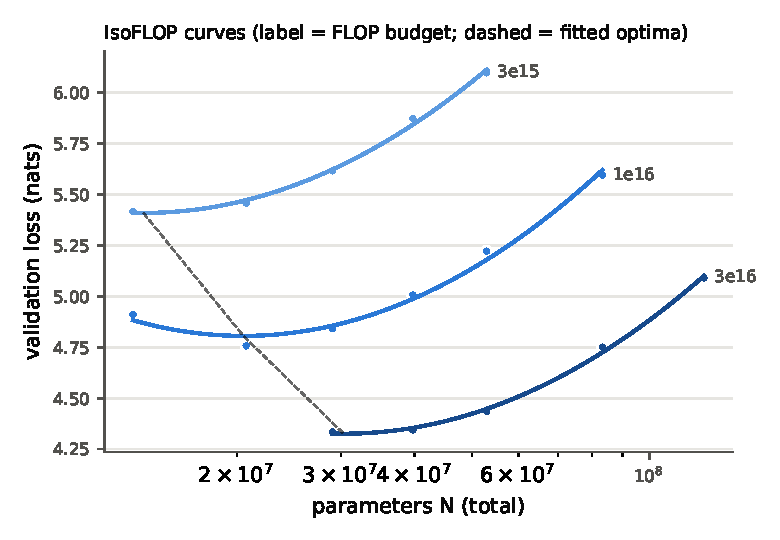
\includegraphics[width=0.75\linewidth]{results/fig_isoflop.pdf}
  \caption{IsoFLOP profiles: validation loss versus parameter count (total-parameter convention) at each FLOP budget. Curves are fitted parabolas in $\log N$; the dashed line connects the fitted minima.}
  \label{fig:isoflop}
\end{figure}

\subsection{Sensitivity to the parameter-counting convention (RQ1)}
Table~\ref{tab:conventions} and Figure~\ref{fig:exponents} report the fitted exponent $a$, the optimal token count $D^*(C_\text{ref})$ and $N^*(C_\text{ref})$ for each approach and convention. \TODO{Report: (i) how much $D^*$ changes across conventions for Approaches 2 and 3 (use \texttt{spreads} in summary.json), (ii) how much the exponent $a$ changes, (iii) whether the bootstrap intervals overlap. Remember Approach~1's $D^*$ is identical across conventions by construction. Then say whether the qualitative conclusion matches Schaeffer et al.}

\begin{table}[t]
  \centering
  \caption{Compute-optimal allocation at $C_\text{ref}$ under each approach and parameter-count convention. $a$ is the exponent in $N^*\propto C^a$. \TODO{Add bootstrap intervals if space allows.}}
  \label{tab:conventions}
  \begin{tabular}{llrrrr}
\toprule
Fit & $N$ convention & exponent $a$ & $D^*$ (M tok) & $N^*$ (M) & $D^*/N^*$ \\
\midrule
Envelope & total & 0.251 & 119 & 24.1 & 4.9 \\
Envelope & non-embedding & 0.674 & 119 & 2.0 & 61.2 \\
Envelope & excl.\ input emb. & 0.276 & 119 & 13.1 & 9.1 \\
IsoFLOP & total & 0.339 & 143 & 20.5 & 7.0 \\
IsoFLOP & non-embedding & 0.985 & 132 & 1.5 & 85.7 \\
IsoFLOP & excl.\ input emb. & 0.419 & 145 & 10.8 & 13.5 \\
Parametric & total & 0.139 & 163 & 18.3 & 8.9 \\
Parametric & non-embedding & 0.380 & 181 & 0.8 & 221.2 \\
Parametric & excl.\ input emb. & 0.160 & 159 & 9.8 & 16.2 \\
\bottomrule
\end{tabular}

\end{table}

\begin{figure}[t]
  \centering
  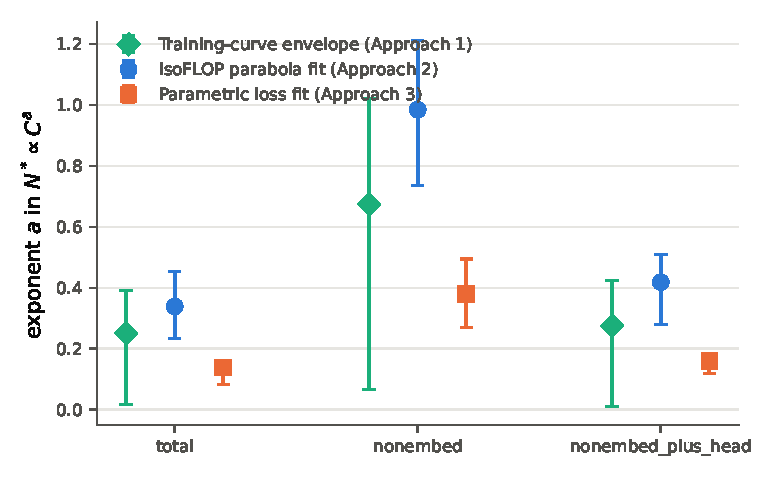
\includegraphics[width=0.75\linewidth]{results/fig_exponents.pdf}
  \caption{Fitted exponent $a$ by convention and approach, with bootstrap 95\% intervals. Intervals reflect which runs are included in the fit, not training-seed variation.}
  \label{fig:exponents}
\end{figure}

\subsection{Structured perturbations of the parameter counts (RQ1)}
Figure~\ref{fig:perturb} shows the optimal tokens-per-parameter ratio and the exponent $a$ under the four perturbations of Section~\ref{sec:perturb}. By construction a multiplicative constant leaves $D^*$ unchanged and rescales $N^*$ and the ratio exactly, so it serves as a check. \TODO{Report, from results/perturbation\_sweep.csv: how the exponent $a$ changes with the additive offset and with the bias slope for each approach (numbers), whether the ratio's trend with compute changes (column ratio\_slope), how large the effect of log-normal noise is relative to the draw-to-draw spread, and whether this agrees in direction with what Schaeffer et al.\ report. Do not claim agreement or disagreement beyond what the numbers show.}

\begin{figure}[t]
  \centering
  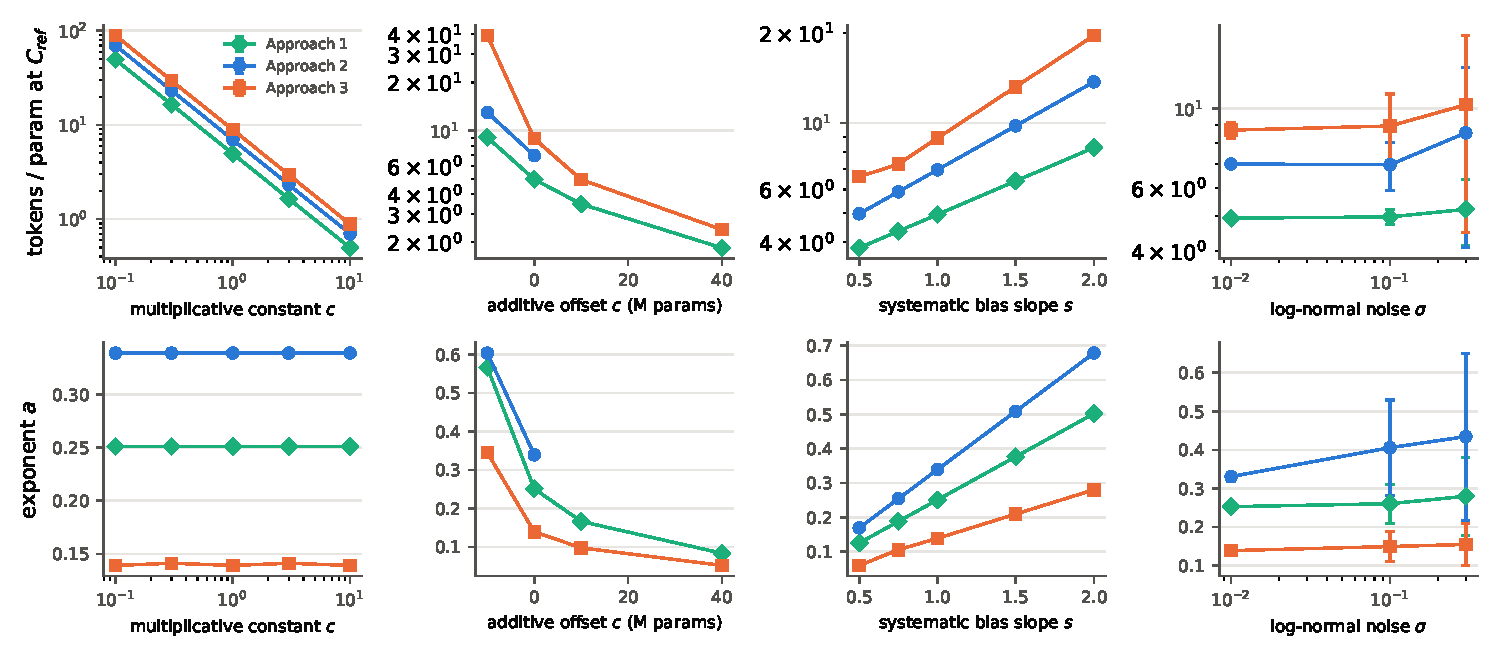
\includegraphics[width=\linewidth]{results/fig_perturbation.pdf}
  \caption{Effect of structured perturbations of the parameter counts (columns: multiplicative, additive, systematic bias, log-normal noise) on the optimal tokens-per-parameter ratio at the reference budget (top) and on the exponent $a$ (bottom), for each approach. Error bars for the noise column are standard deviations over 10 draws.}
  \label{fig:perturb}
\end{figure}

\subsection{Comparison of the three approaches (RQ3)}
\TODO{Use \texttt{approach\_gap} in summary.json: for each convention, the gap in $a$ and the relative gap in $D^*$ between each pair of approaches. State which pair agrees best and which worst, with numbers.}

\subsection{Shrinking the fitting grid (RQ2)}
Figure~\ref{fig:shrink} shows the spread of the exponent across conventions as the grid shrinks. \TODO{Using shrink\_sweep.csv, state whether the spread grows when budgets or sizes are removed, and at what point a fit fails entirely (no interior minimum, fewer than two valid budgets). If there is no clear trend with this few subsets, say so plainly.}

\begin{figure}[t]
  \centering
  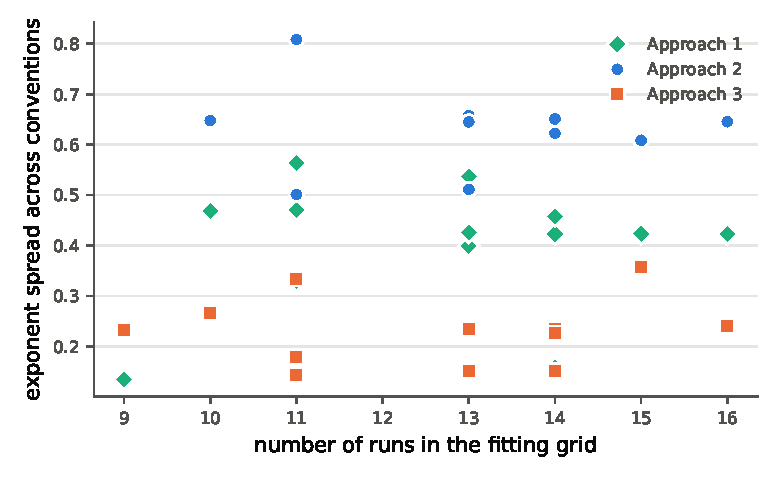
\includegraphics[width=0.75\linewidth]{results/fig_shrink.pdf}
  \caption{Spread of the exponent $a$ across parameter-count conventions for each subset of the grid, against the number of runs retained.}
  \label{fig:shrink}
\end{figure}
